\chapter{Supplementary data to \Chapref{STD_paper}}
%\chapter{Supplementary Information to \Chapref{Longevity}}%labstudy is the label for chapter 2.
\label{chap:Appendix_STD}

\bigskip
\medskip
\begin{center}

\noindent{\Large \bf Mammalian morphological diversity does not increase in response to the Cretaceous-Paleogene mass extinction and the extinction of the (non-avian) dinosaurs} \\
\bigskip
\end{center}

This section (Fig \ref{Supp_Mammaliaformes_rarefied} and \ref{Supp_Eutheria_rarefied}) contains the rarefied results of the Mammaliaformes and Eutheria datasets

\begin{figure}
\centering
    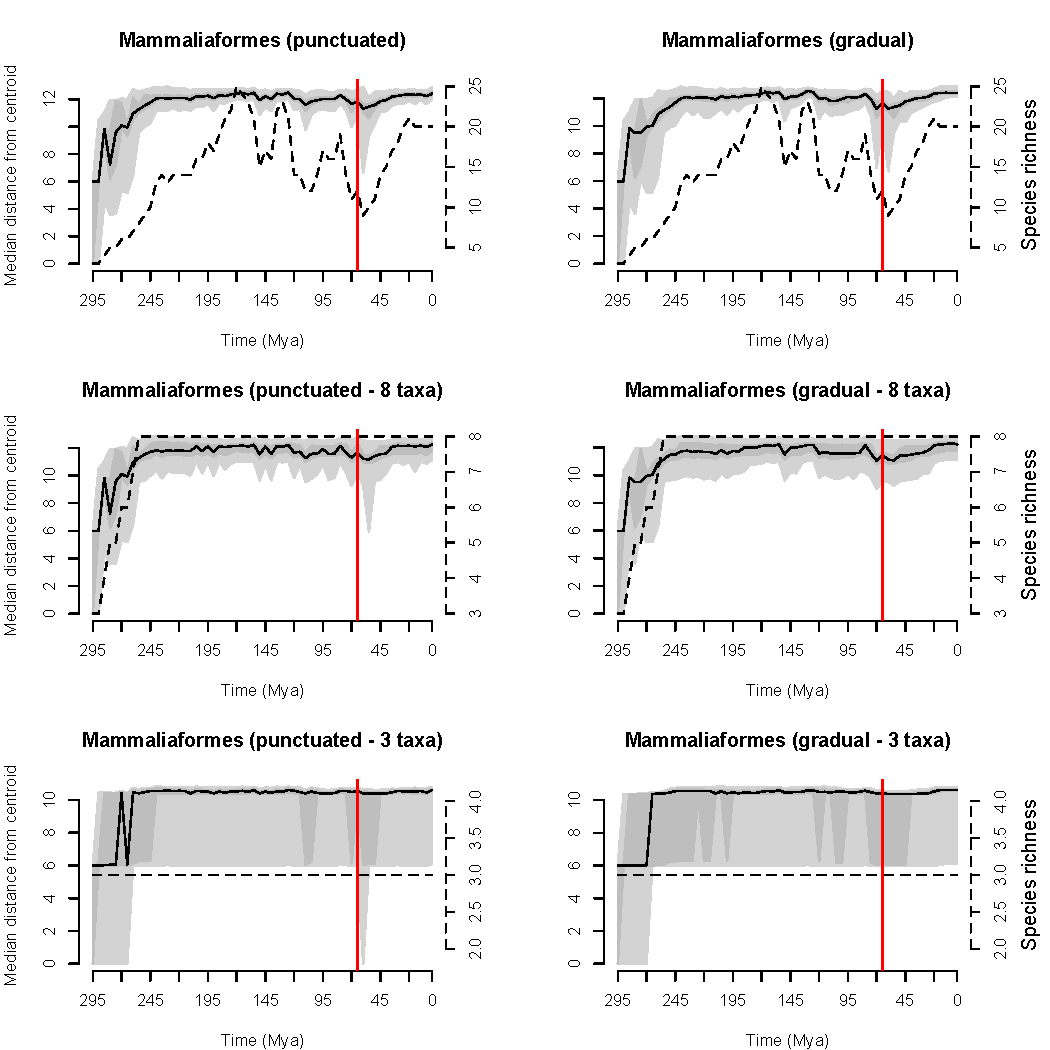
\includegraphics[keepaspectratio=true]{Supplementaries/Figures/STD/Slater_full.pdf}
\caption[Mammaliaformes disparity (rarefied)]{Observed and rarefied variation of disparity through time among Mammaliaformes with a punctuated or gradual evolution model. The x axis represents the time in Million of years ago (Mya). The y axis represents the disparity measured as the median distance from centroid per sub-sample. The solid black lines is the mean disparity; the confidence intervals (CI) are represent by the grey polygons (50\% CI in dark grey and 95\% CI in light grey). The dashed line represent the species richness in each sub-sample (values are reported on the right hand side of each graphs). The red vertical line represents the K-Pg boundary (66 Mya).}
\label{Supp_Mammaliaformes_rarefied}
\end{figure}

\begin{figure}
\centering
    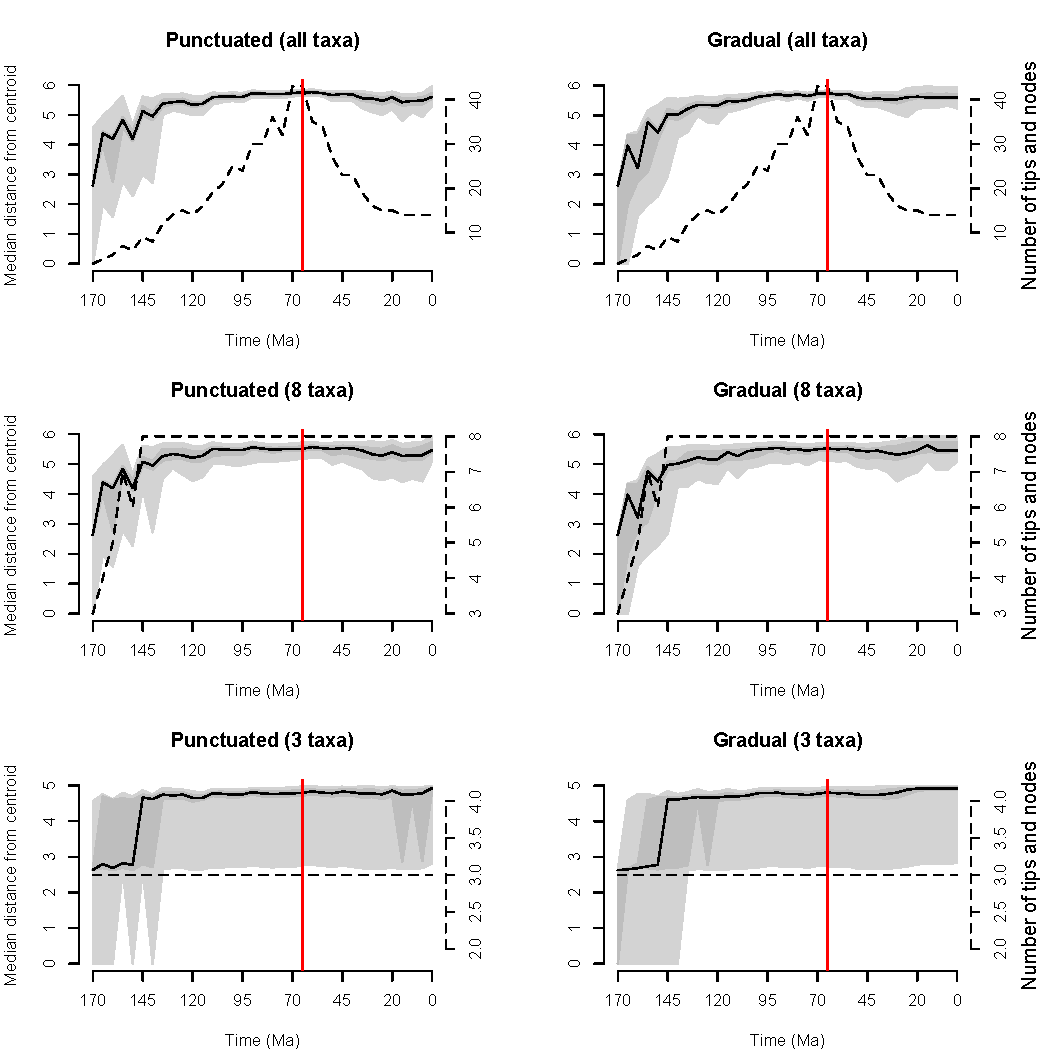
\includegraphics[keepaspectratio=true]{Supplementaries/Figures/STD/Rarefaction-beck.pdf}
\caption[Eutheria disparity (rarefied)]{Variations of disparity through time among Eutherian with a punctuated or gradual evolution model for different number of taxa (rarefaction). The x axis represents the time in Million of years ago (Mya). The y axis represents the disparity measured as the median distance from centroid per sub-sample. The solid black lines is the mean disparity; the confidence intervals (CI) are represent by the grey polygons (50\% CI in dark grey and 95\% CI in light grey). The dashed line represent the species richness in each sub-sample (values are reported on the right hand side of each graphs). The red vertical line represents the K-Pg boundary (66 Mya).}
\label{Supp_Eutheria_rarefied}
\end{figure}

\newpage
This section (Fig \ref{Supp_disparity_all_Mammaliaformes}, \ref{Supp_disparity_all_Eutheria}, \ref{Supp_disparity_all_Mammaliaformes_rarefied} and \ref{Supp_disparity_all_Eutheria_rarefied}) contains the results of the analysis of the Mammaliaformes and Eutherian data set with all the disparity measurements and methods for sampling disparity through time.
The different disparity measurements are the median distance from centroid (see methods section in the main text for details) as well as the median sum and products of ranges and variances from \cite{Wills1994}.
The different methods for sampling disparity through time are:
\begin{enumerate}
\item \textbf{Intervals (tips only)}. We selected every tips present at every stages from the early Middle Jurassic (Bajocian, starting at 170.3 Mya) to the present. We collapsed together every stage containing less than 3 tips. Note that some tips where present in multiple stages due to their occurrence data (see methods section in the main text for details on the occurrence data).
\item \textbf{Intervals (tips and nodes)}. We selected every stage tips and nodes present at every stages from the early Middle Jurassic (Bajocian, starting at 170.3 Mya) to the present. We collapsed together every stage containing less than 3 elements (tips and/or nodes).
\item \textbf{Slices (punctuated)}. These are the results presented in the main text where time is sample equidistantly and evolution is assumed to be punctuated (randomly selecting either data from the descendant or the ancestor when slicing through a branch; see methods section in the main text for details).
\item \textbf{Slices (punctuated: acctran)}. Similar as slices (punctuated) method but data is always selected from the descendant (see methods section in the main text for details).
\item \textbf{Slices (punctuated: deltran)}. Similar as slices (punctuated) method but data is always selected from the ancestor (see methods section in the main text for details).
\item \textbf{Slices (gradual)}. SThese are the results presented in the main text where time is sample equidistantly and evolution is assumed to be gradual (data is selected from the descendant or the ancestor based on branch length; see methods section in the main text for details).
\end{enumerate}
We also rarefied both data sets for all the metrics and all the methods using only 3 taxa for the interval methods and 8 taxa for the slices methods.


\begin{landscape}
\begin{figure}[!htbp]
\centering
    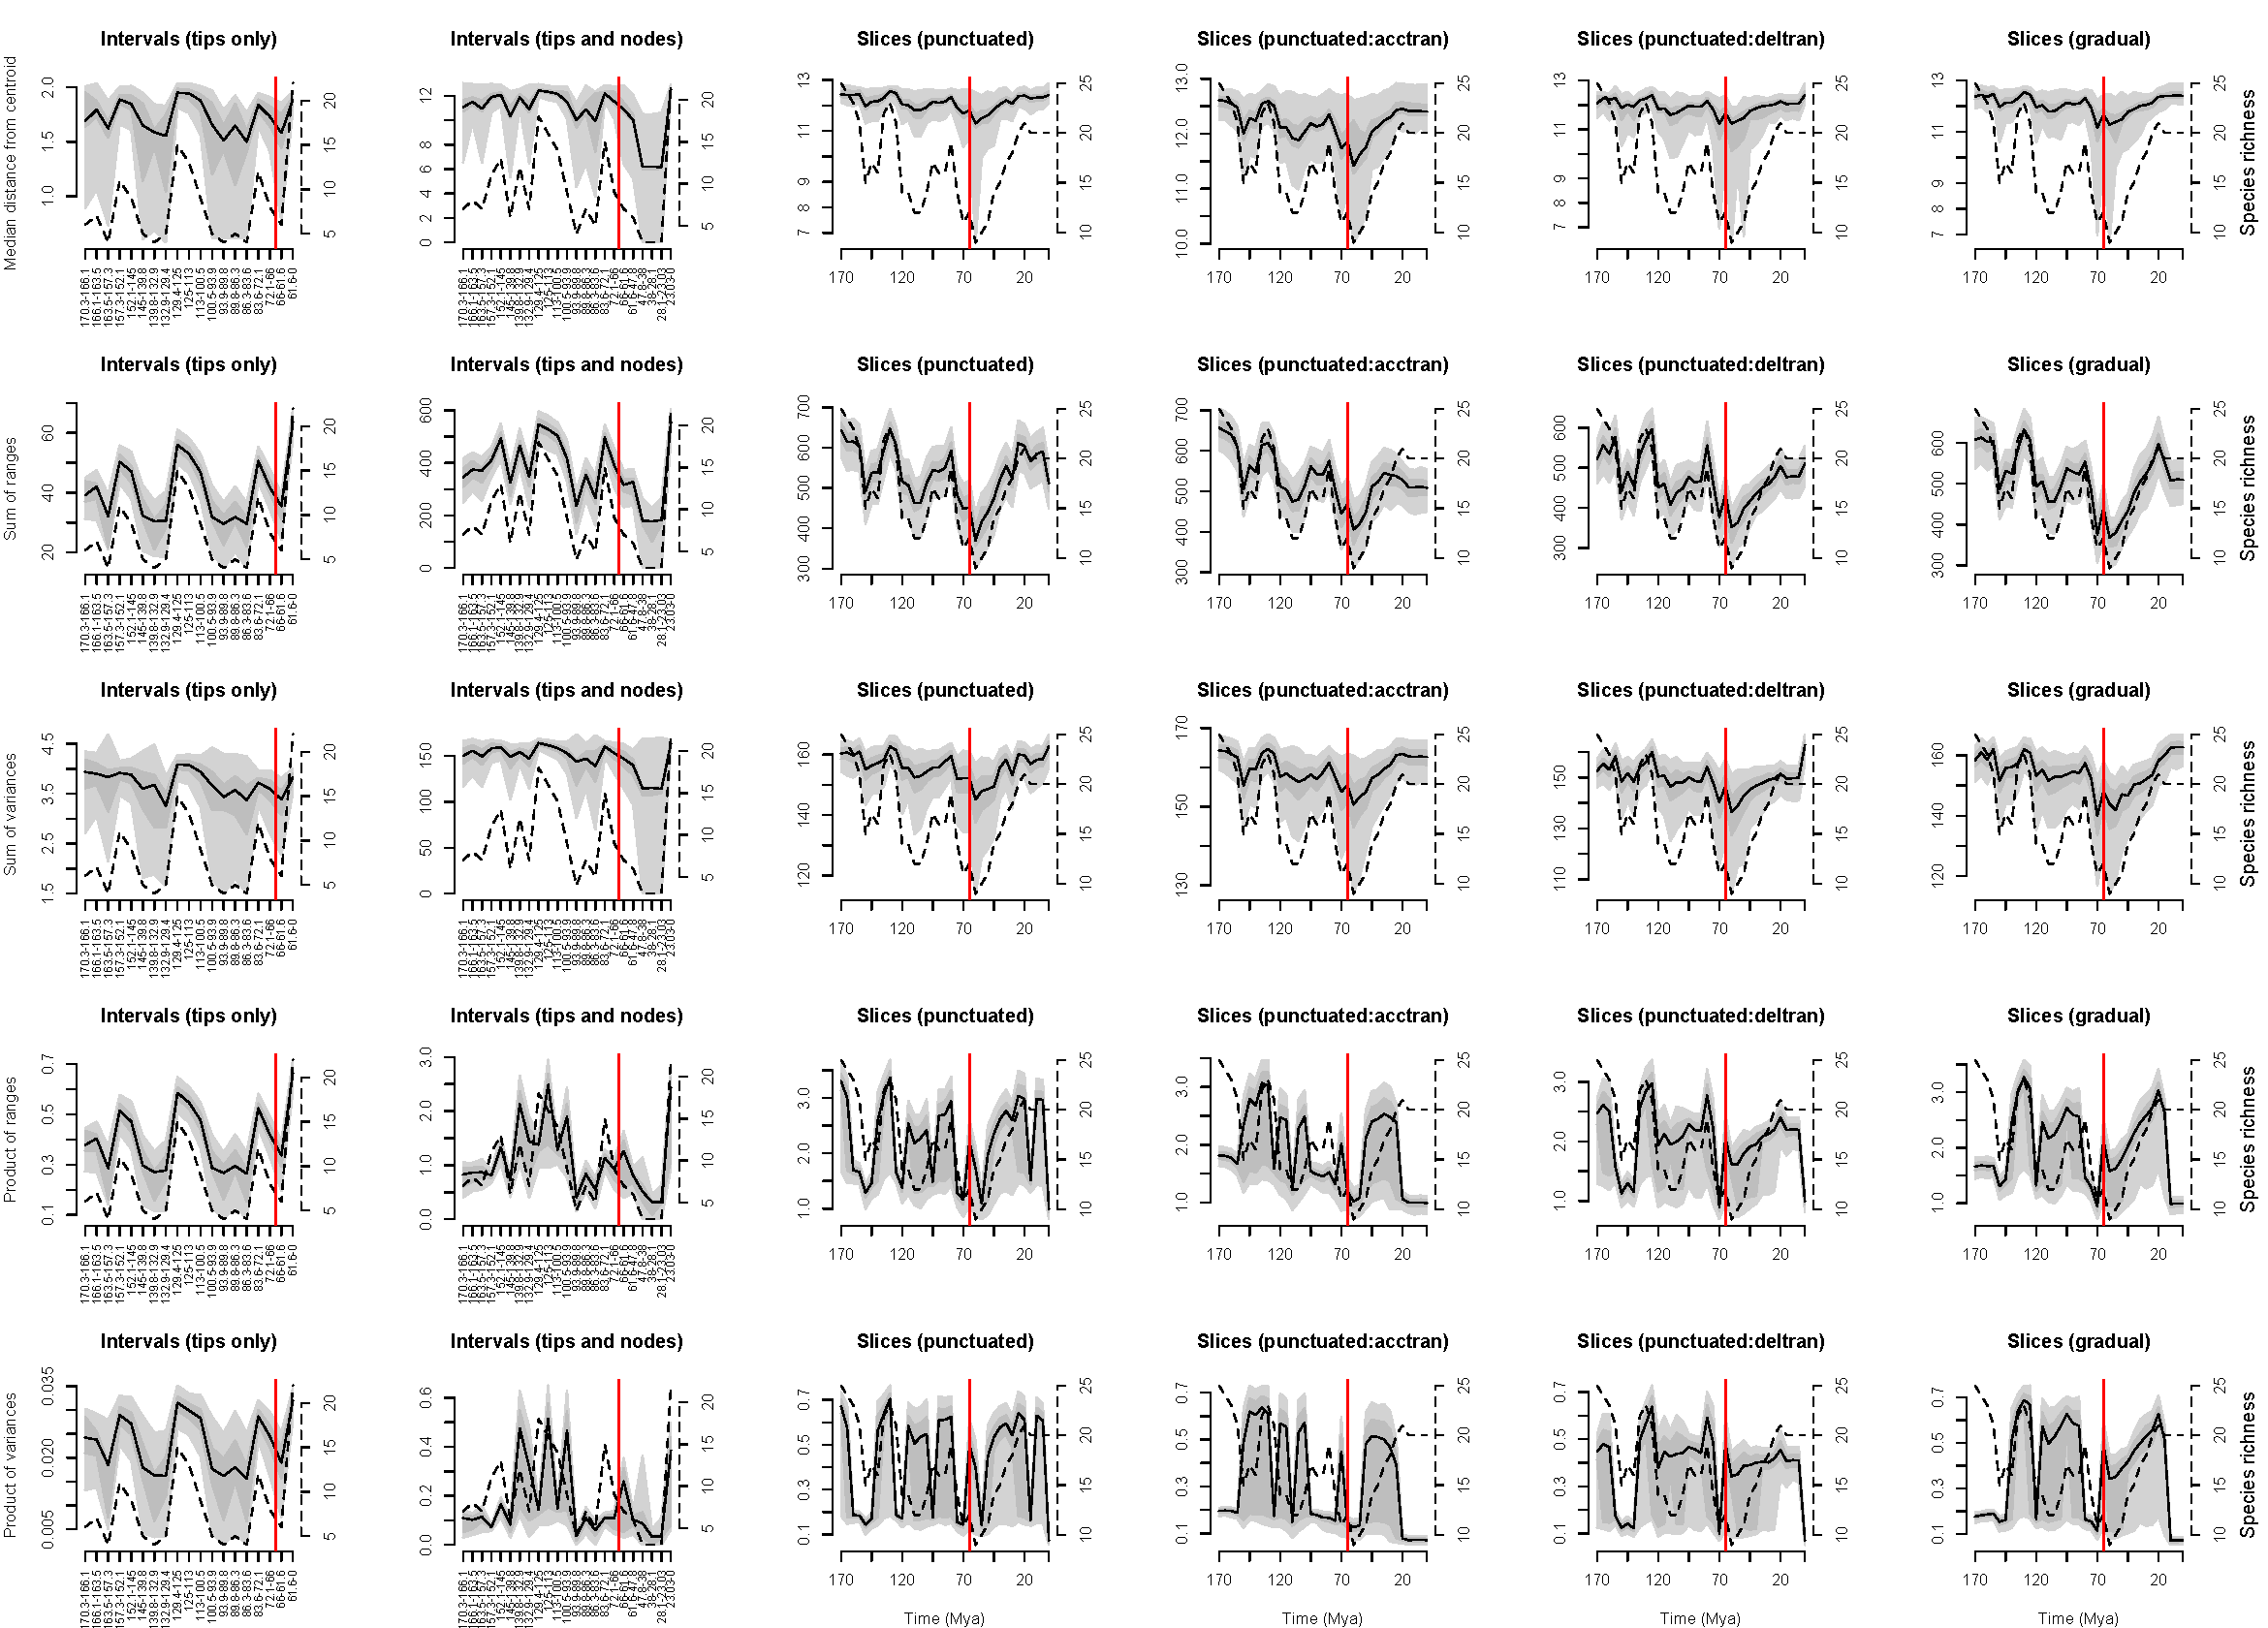
\includegraphics[width=\textwidth,height=\textheight,keepaspectratio]{Supplementaries/Figures/STD/Mammaliaformes_all_methods.pdf}
\caption[Comparison of all the disparity metrics and all the time series methods for Mammaliaformes]{Variations of disparity through time among Mammaliaformes with disparity measurements and methods for sampling disparity through time. The x axis represents the time in Million of years ago (Mya). The y axis represents the disparity measured as the median distance from centroid per sub-sample. The solid black lines is the mean disparity; the confidence intervals (CI) are represent by the grey polygons (50\% CI in dark grey and 95\% CI in light grey). The dashed line represent the species richness in each sub-sample (values are reported on the right hand side of each graphs). The red vertical line represents the K-Pg boundary (66 Mya).}
\label{Supp_disparity_all_Mammaliaformes}
\end{figure}
\end{landscape}

\begin{landscape}
\begin{figure}[!htbp]
\centering
    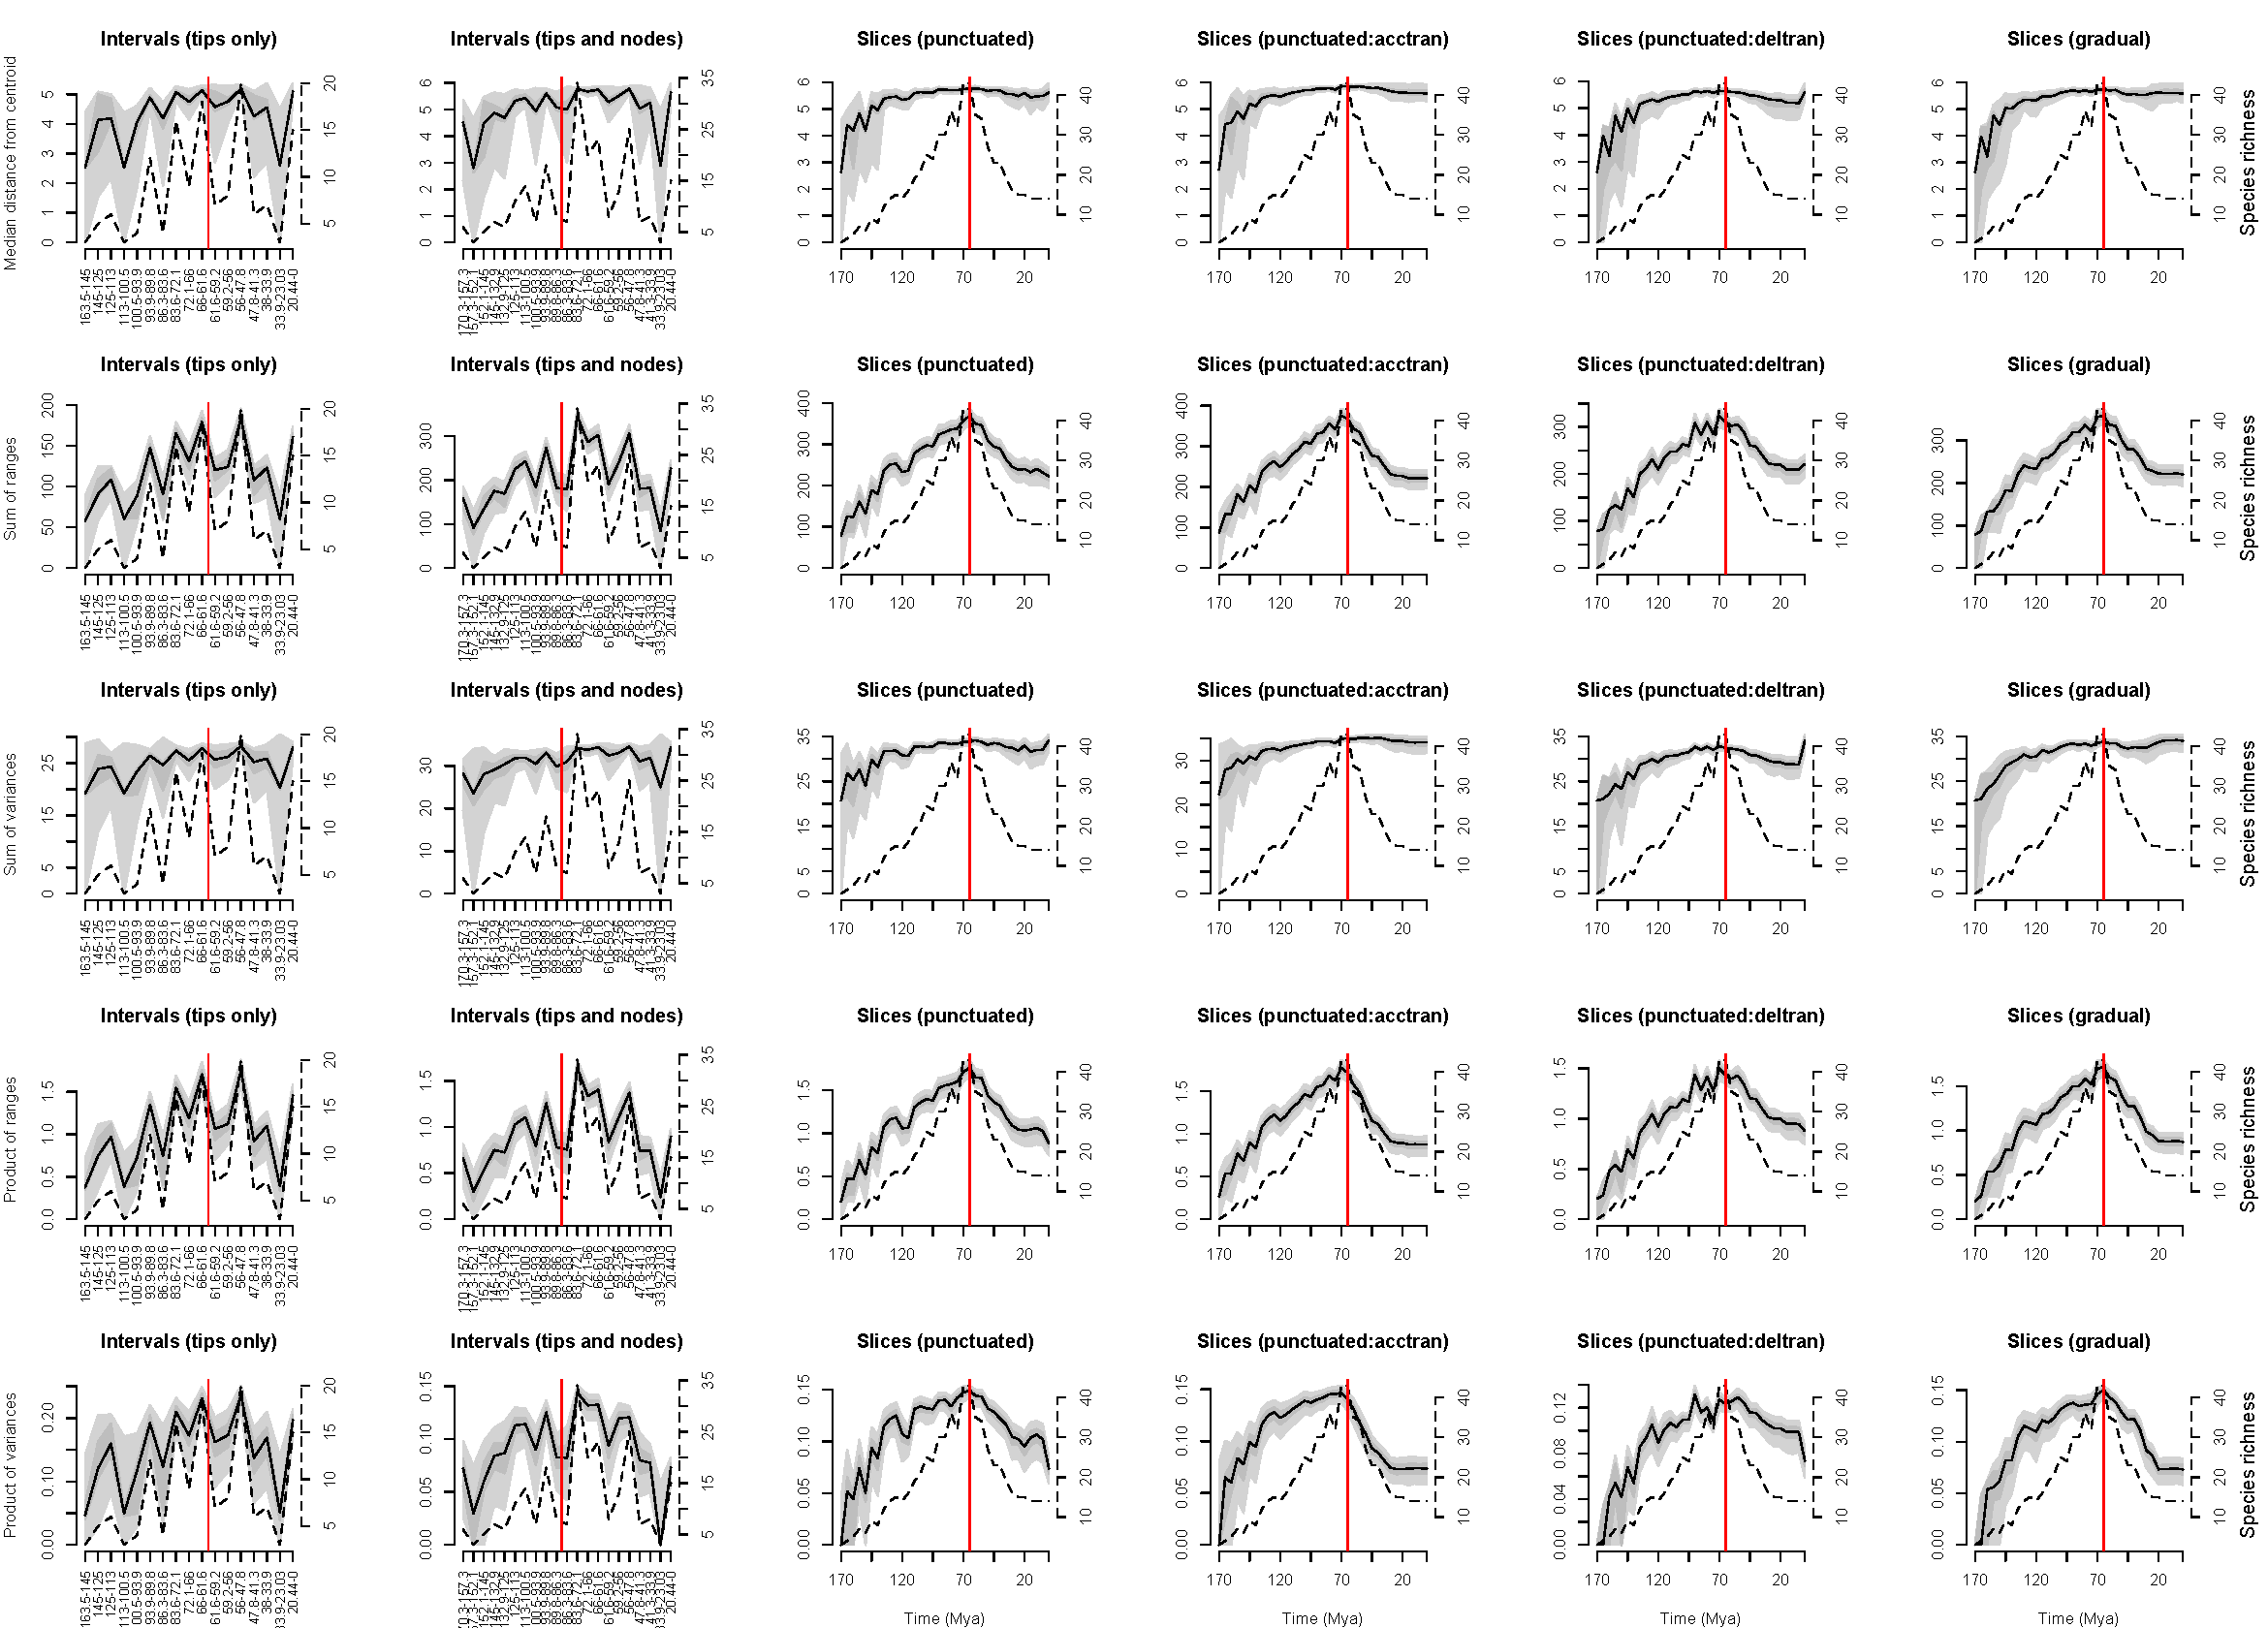
\includegraphics[width=\textwidth,height=\textheight,keepaspectratio]{Supplementaries/Figures/STD/Eutheria_all_methods.pdf}
\caption[Comparison of all the disparity metrics and all the time series methods for Eutheria]{Variations of disparity through time among Eutherian with disparity measurements and methods for sampling disparity through time. The x axis represents the time in Million of years ago (Mya). The y axis represents the disparity measured as the median distance from centroid per sub-sample. The solid black lines is the mean disparity; the confidence intervals (CI) are represent by the grey polygons (50\% CI in dark grey and 95\% CI in light grey). The dashed line represent the species richness in each sub-sample (values are reported on the right hand side of each graphs). The red vertical line represents the K-Pg boundary (66 Mya).}
\label{Supp_disparity_all_Eutheria}
\end{figure}
\end{landscape}



\begin{landscape}
\begin{figure}[!htbp]
\centering
    \includegraphics[width=\textwidth,height=\textheight,keepaspectratio]{Supplementaries/Figures/STD/Mammaliaformes_all_methods_rarefied.pdf}
\caption[Comparison of all the disparity metrics and all the time series methods for Mammaliaformes (rarefied)]{Variations of disparity through time among Mammaliaformes with disparity measurements and methods for sampling disparity through time (rarefied with 3 taxa for the interval method and 8 taxa for the slice method). The x axis represents the time in Million of years ago (Mya). The y axis represents the disparity measured as the median distance from centroid per sub-sample. The solid black lines is the mean disparity; the confidence intervals (CI) are represent by the grey polygons (50\% CI in dark grey and 95\% CI in light grey). The dashed line represent the species richness in each sub-sample (values are reported on the right hand side of each graphs). The red vertical line represents the K-Pg boundary (66 Mya).}
\label{Supp_disparity_all_Mammaliaformes_rarefied}
\end{figure}
\end{landscape}

\begin{landscape}
\begin{figure}[!htbp]
\centering
    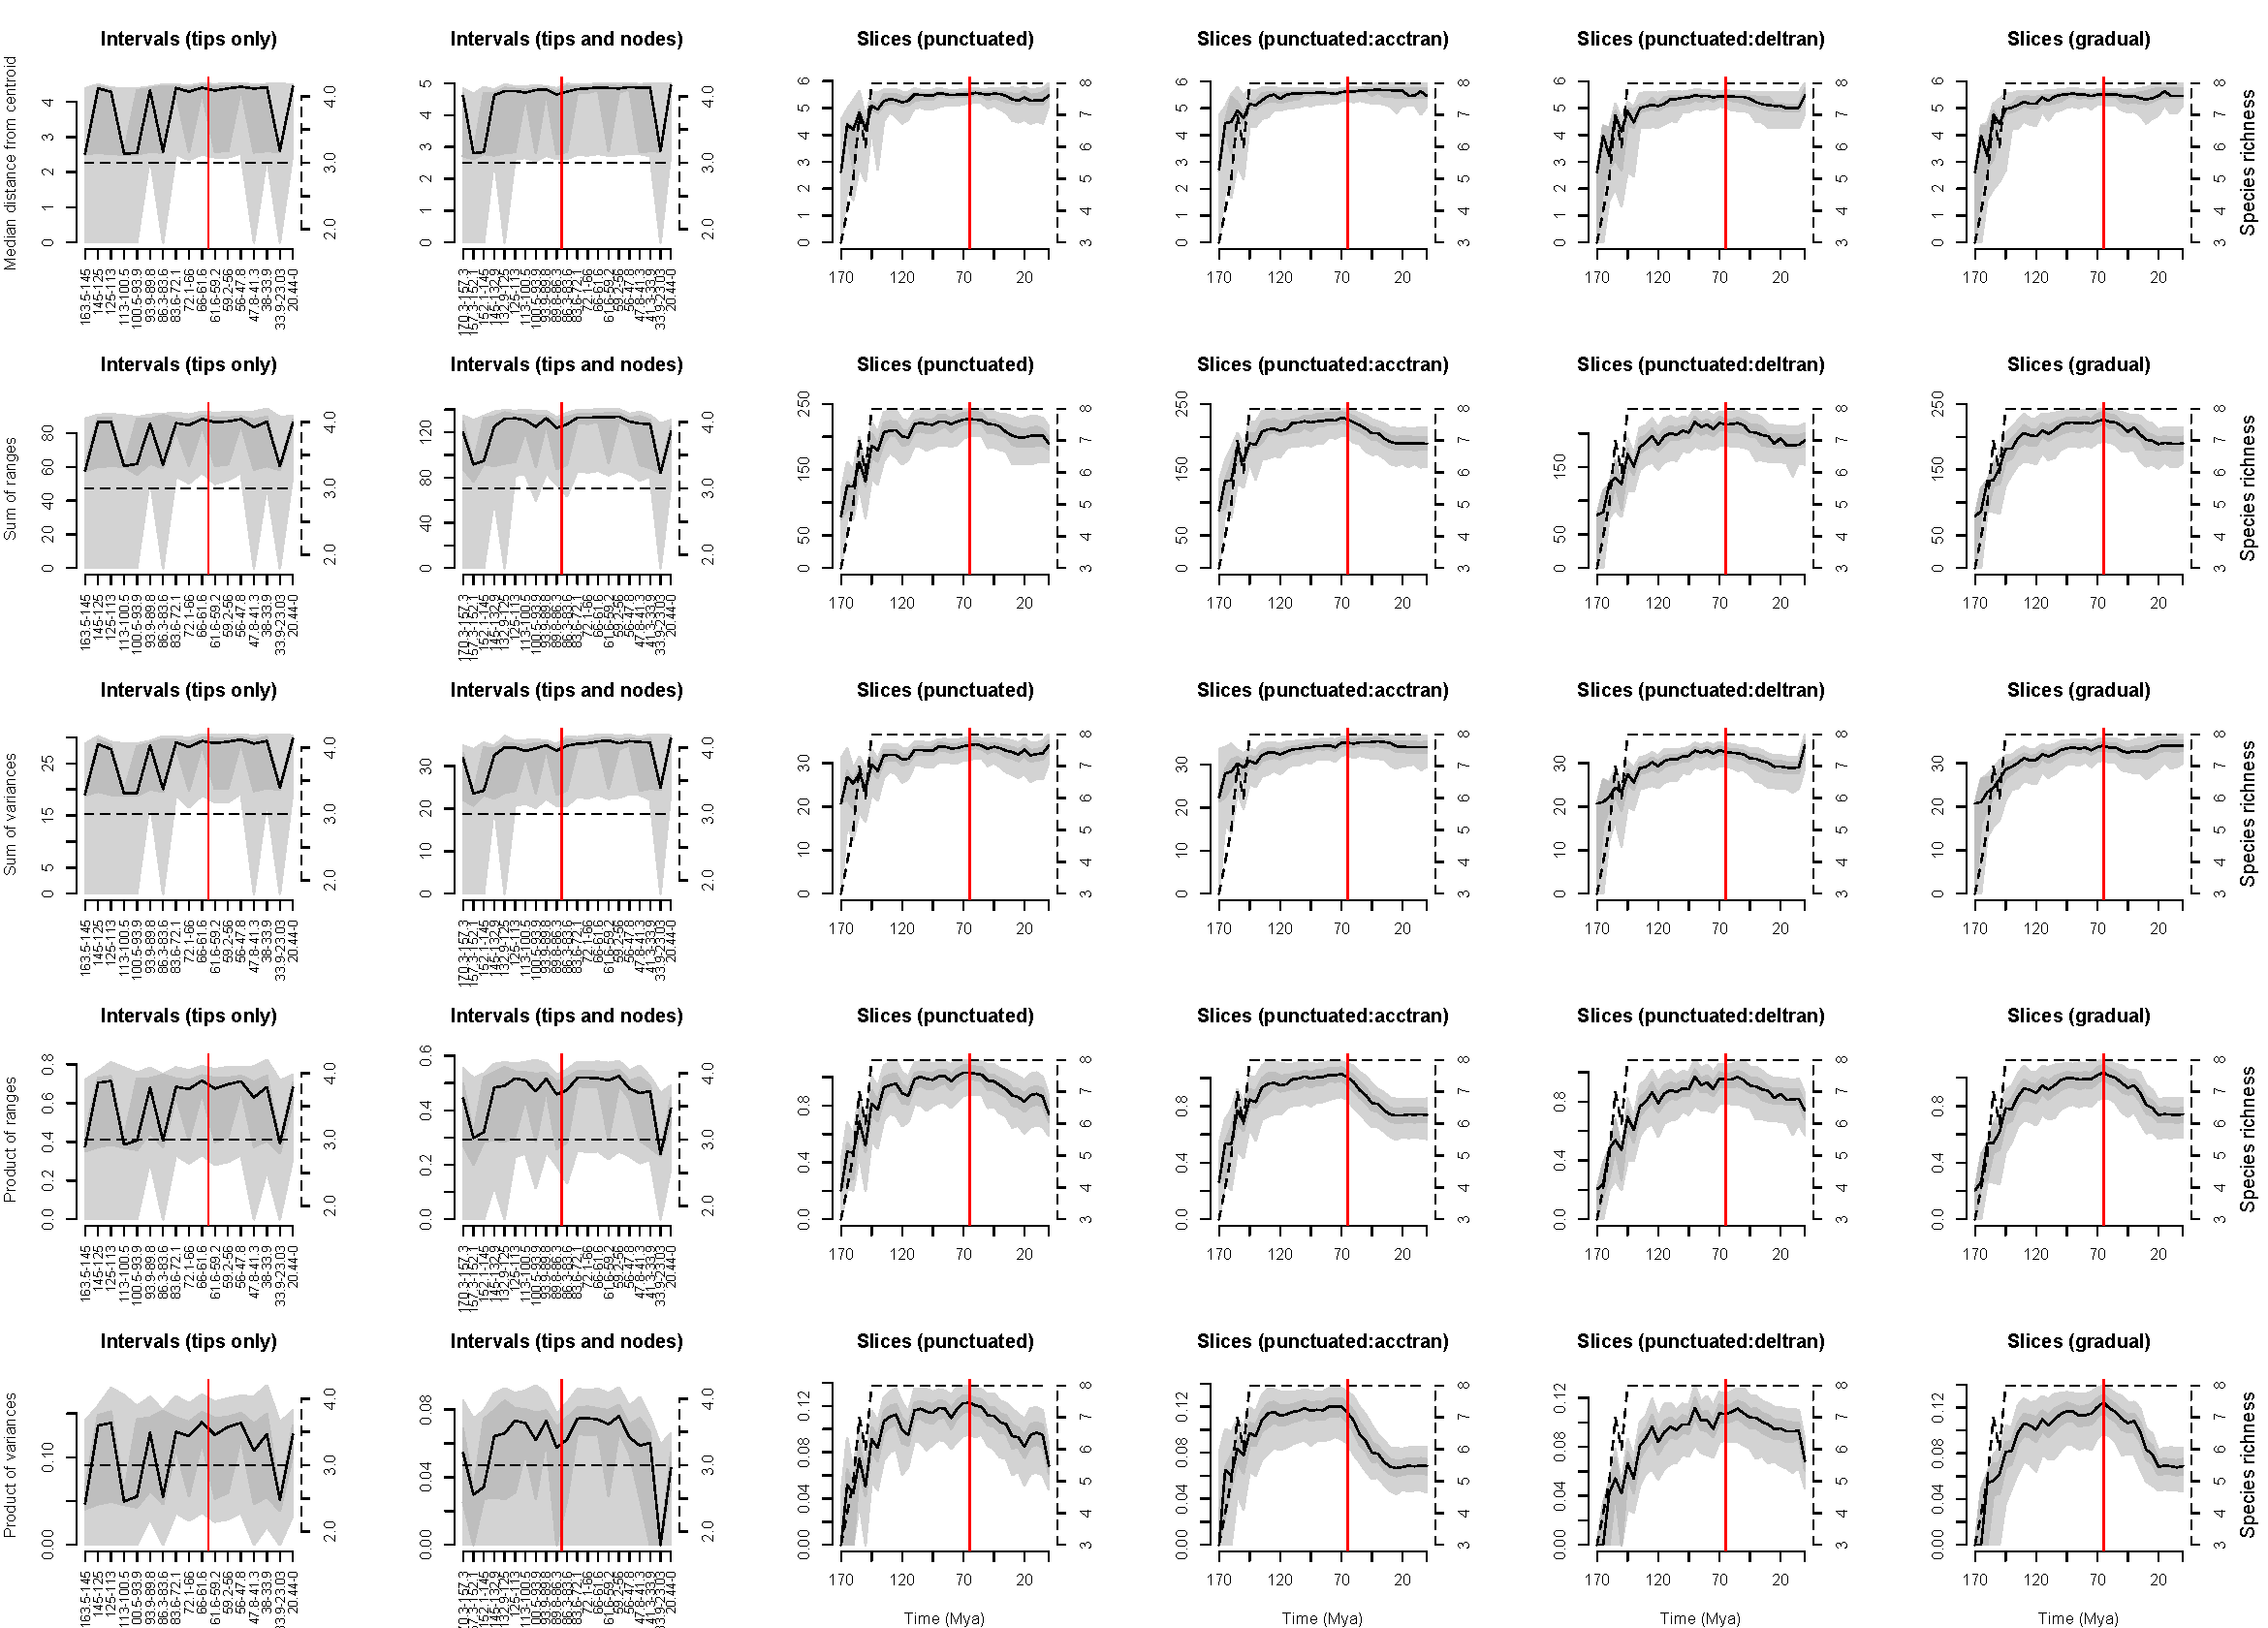
\includegraphics[width=\textwidth,height=\textheight,keepaspectratio]{Supplementaries/Figures/STD/Eutheria_all_methods_rarefied.pdf}
\caption[Comparison of all the disparity metrics and all the time series methods for Eutheria (rarefied)]{Variations of disparity through time among Eutherian with disparity measurements and methods for sampling disparity through time (rarefied with 3 taxa for the interval method and 8 taxa for the slice method). The x axis represents the time in Million of years ago (Mya). The y axis represents the disparity measured as the median distance from centroid per sub-sample. The solid black lines is the mean disparity; the confidence intervals (CI) are represent by the grey polygons (50\% CI in dark grey and 95\% CI in light grey). The dashed line represent the species richness in each sub-sample (values are reported on the right hand side of each graphs). The red vertical line represents the K-Pg boundary (66 Mya).}
\label{Supp_disparity_all_Eutheria_rarefied}

\end{figure}
\end{landscape}